\documentclass[12pt, a4]{article}
\usepackage[english]{babel}
\usepackage[utf8]{inputenc}
\usepackage[a4paper, total={16cm, 24cm}]{geometry}

\usepackage{graphicx}
\graphicspath{ {./screenshots/} }

\usepackage{fancyhdr}
\pagestyle{fancy}
\fancyhf{}
\lhead{Data Mining and Business Intelligence}
\rhead{Mini Project}
\rfoot{\thepage}

\usepackage{hyperref}
\makeatletter
\g@addto@macro{\UrlBreaks}{\UrlOrds}
\makeatother
\usepackage[section]{placeins}

\title{
  \vspace{-1.0cm}
  \textbf{Logistic Regression with Rust}
}
\author{
  Arpit Bhat\\
  \textit{501808}
  \and
  Archit Bhonsle\\
  \textit{501810}
  \and
  Shalmali Kulkarni\\
  \textit{501835}
}
\date{}

\begin{document}

\maketitle
\thispagestyle{fancy}

\section{Problem Statement}

We aim to create a desktop application using GTK, a toolkit to create GUI apps
that guides use through the a simplified version of the machine learning pipeline. The algorithm we'll be using is logistic regression which is used in
various simple classification tasks.

\section{Dataset}

The dataset we've chosen is reduced version of a larger dataset with 76
attributes found here:
\url{https://archive.ics.uci.edu/ml/datasets/Heart+Disease}.
This reduced dataset has 14 attributes (described in detail in table
\ref{table:attributes}) and one target variable which indicates whether heart
disease is present or not. The reduced dataset has numeric, discrete,
continuous and binary attributes all of which can be represented as numbers
which in our case are 64-bit floating point values. This is an assumption that helps us optimize our model and skip certain steps like mapping nominal attributes to unique numbers.

\begin{table}[h]
\centering
\begin{tabular}{| l | l |}
  \hline
  Column   & Attribute                                            \\
  \hline
  age      & Age in years                                         \\
  sex      & Sex of person: 0 is female, 1 is male                \\
  cp       & Chest pain type                                      \\
  trestbps & Resting blood pressure (in mm Hg)                    \\
  chol     & Serum cholesterol in mg/dl                           \\
  fbs      & 1 if fasting blood sugar $>$ 120 mg/dl else 0        \\
  restecg  & Resting electrocardiograph results                   \\
  thalch   & Maximum heart rate achieved (in mm Hg)               \\
  exang    & 1 if exercise induced angina else 0                  \\
  oldpeak  & ST depression induced by exercise relative to rest   \\
  slope    & The slope of the peak exercise ST segment            \\
  ca       & Number of major vessels (0-3) colored by fluoroscope \\
  thal     & 3 = normal; 6 = fixed defect; 7 = reversable defect  \\
  target   & 1 if heart disease is present 0 otherwise            \\
  \hline
\end{tabular}
\caption{Attributes in the heart dataset}
\label{table:attributes}
\end{table}

\section{Model}

The model we use here is
\href{https://en.wikipedia.org/wiki/Logistic_regression}{logistic regression}.
It is a model used for binary classification problems like the heart disease
problem we are tackling here. A fundamental part of this model is the sigmoid function which maps an arbitary number of real values to a probability between 0 and 1:

\[ \frac{1}{1 + e^{-x}} \]

The cost function we use is:

\[ J(\theta) = \frac{1}{m} \sum_{i = 1}^{m}
  \left(
    y^{(i)}\log\left(h_{\theta}(x^{(i)})\right) +
    \left(1 - y^{(i)}\right)\log\left(1 - h_{\theta}(x^{(i)})\right)
  \right)
\]

And thus in gradient descent, which is basically applying this repeatedly:

\[
  \theta_{j} := \theta_{j} -
  \alpha \frac{\delta}{\delta\theta_{j}} J(\theta)
\]

becomes after resolving the derivative using calculus:

\[
  \theta_{j} := \theta_{j} -
  \frac{\alpha}{m} \sum_{i = 1}^{m} x_{j}^{(i)}
  \left(h_{\theta}(x^{(i)}) - y^{(i)} \right)
\]

\

\section{Creating the model and testing}

The core code for the model is encapsulated inside the following
\texttt{forward\_backward} function:

\begin{verbatim}
fn forward_backward(
    weights: &Array2<f64>,
    bias: &f64,
    x_train: &Array2<f64>,
    y_train: &Array2<f64>,
) -> (f64, Array2<f64>, f64) {
    // forward
    let y_head: Array2<f64> = sigmoid(weights.t().dot(x_train)
        .mapv(|x| x + bias));
    let loss = (y_train * &(y_head.mapv(|z| z.ln()))
        + &((y_train.mapv(|z| 1. - z)) * &y_head.mapv(|z| (1. - z).ln())))
        .mapv(|z| -1. * z);
    let cost = loss.sum() / x_train.ncols() as f64;

    // backward
    let d_weights = (x_train.dot(&(&y_head - y_train).t()))
        .mapv(|z| z / x_train.ncols() as f64);
    let d_bias = (&y_head - y_train).sum() / x_train.ncols() as f64;

    (cost, d_weights, d_bias)
}
\end{verbatim}

Here, \texttt{y\_head} is $h_{\theta}(x^{(i)})$ or the hypothesis. \texttt{loss}
is $J(\theta)$ and \texttt{cost} is the average loss. This comprises the
``forward'' step. In the backward step we calculate the change in the weights,
\texttt{d\_weights} and the change in bias as \texttt{d\_bias}.

These values are then used by the \texttt{update} function which tweaks the
weights and the biases for the specified \texttt{iterations}. Thus, the model
is trained.

\begin{verbatim}
fn update(
    weights: Array2<f64>,
    bias: f64,
    x_train: Array2<f64>,
    y_train: Array2<f64>,
    learning_rate: f64,
    iterations: usize,
) -> (Vec<f64>, Array2<f64>, f64) {
    let mut costs: Vec<f64> = Vec::new();
    let mut weights = weights;
    let mut bias = bias;

    for _ in 0..iterations {
        let (cost, d_weight, d_bias) = forward_backward(
            &weights, &bias, &x_train, &y_train);
        weights -= &d_weight.mapv(|x| learning_rate * x);
        bias -= learning_rate * d_bias;

        costs.push(cost);
    }

    (costs, weights, bias)
}
\end{verbatim}

\section{Using the application}

The application has three pages. Each page has represents one section of the
machine learning pipeline.

\begin{enumerate}
  \item{In the first step, as shown in figure \ref{fig:choose}, we select our
        dataset. We can we review it in the tabular view and inspect it's
        various attributes.}
  \item{After that we perform preprocessing on this data. As one may observe
        in the tabular view some attributes go in the high 100s while some
        are simple binary values, 0 and 1. If we give this data to the model
        it may cause problems. To counter this we normalize the data. This is
        demonstrated in figure \ref{fig:preprocessing}.}
  \item{In the third step, as shown in the figure \ref{fig:model}, we actually
        train our model. We specify the learning rate and the number of
        iterations. Once trained a graph of the model's cost as the it goes
        through various iterations is graphed. Based on this we can evaluate
        the model. Once trained we can test the model against the testing data.
        Then the various metrics like accuracy, precision, recall and f1-score
        are shown.}
\end{enumerate}

\begin{figure}[h]
\centering
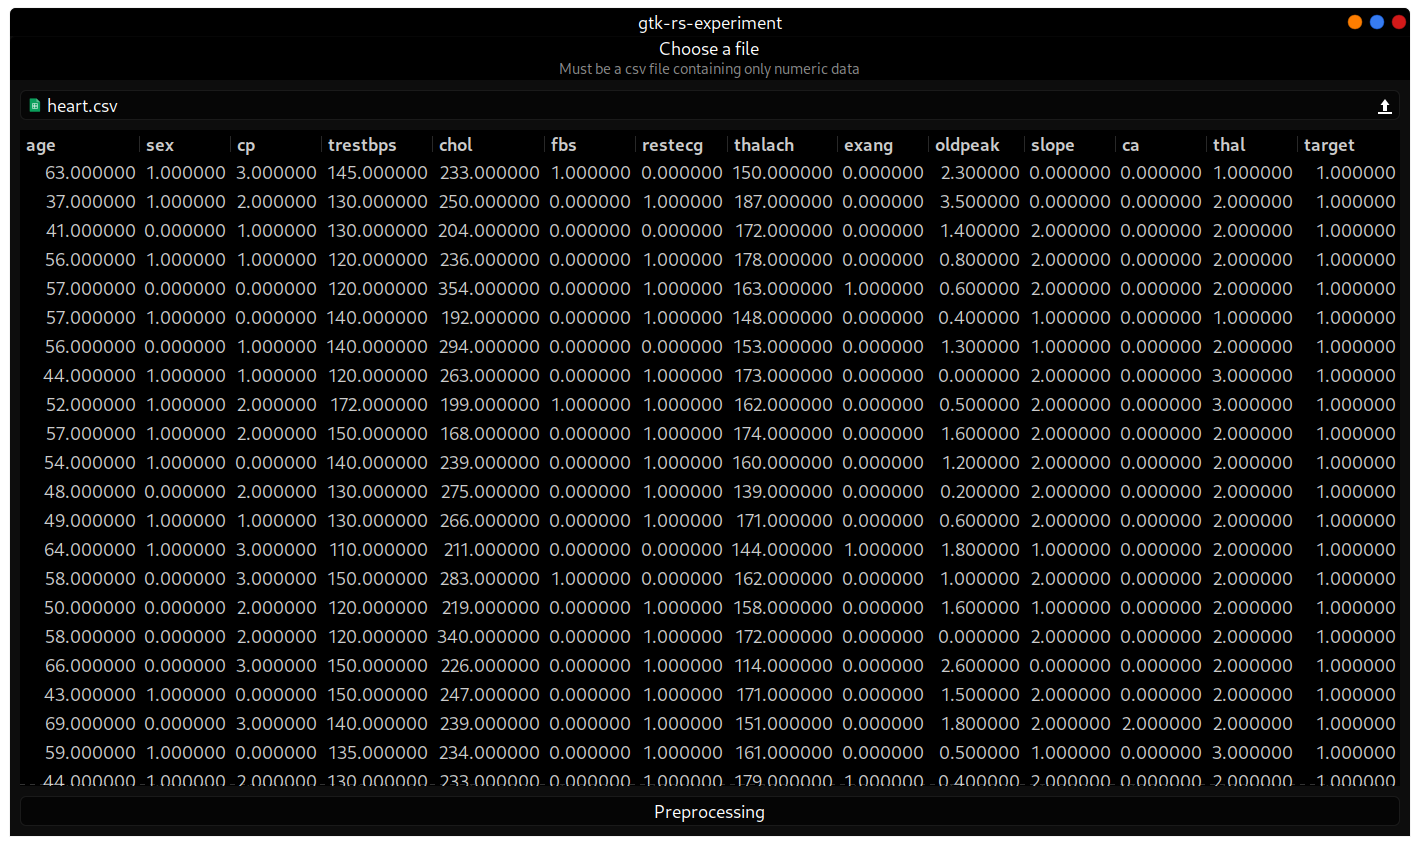
\includegraphics[width=120mm]{choose}
\caption{Choose Page}
\label{fig:choose}
\end{figure}


\begin{figure}[h]
\centering
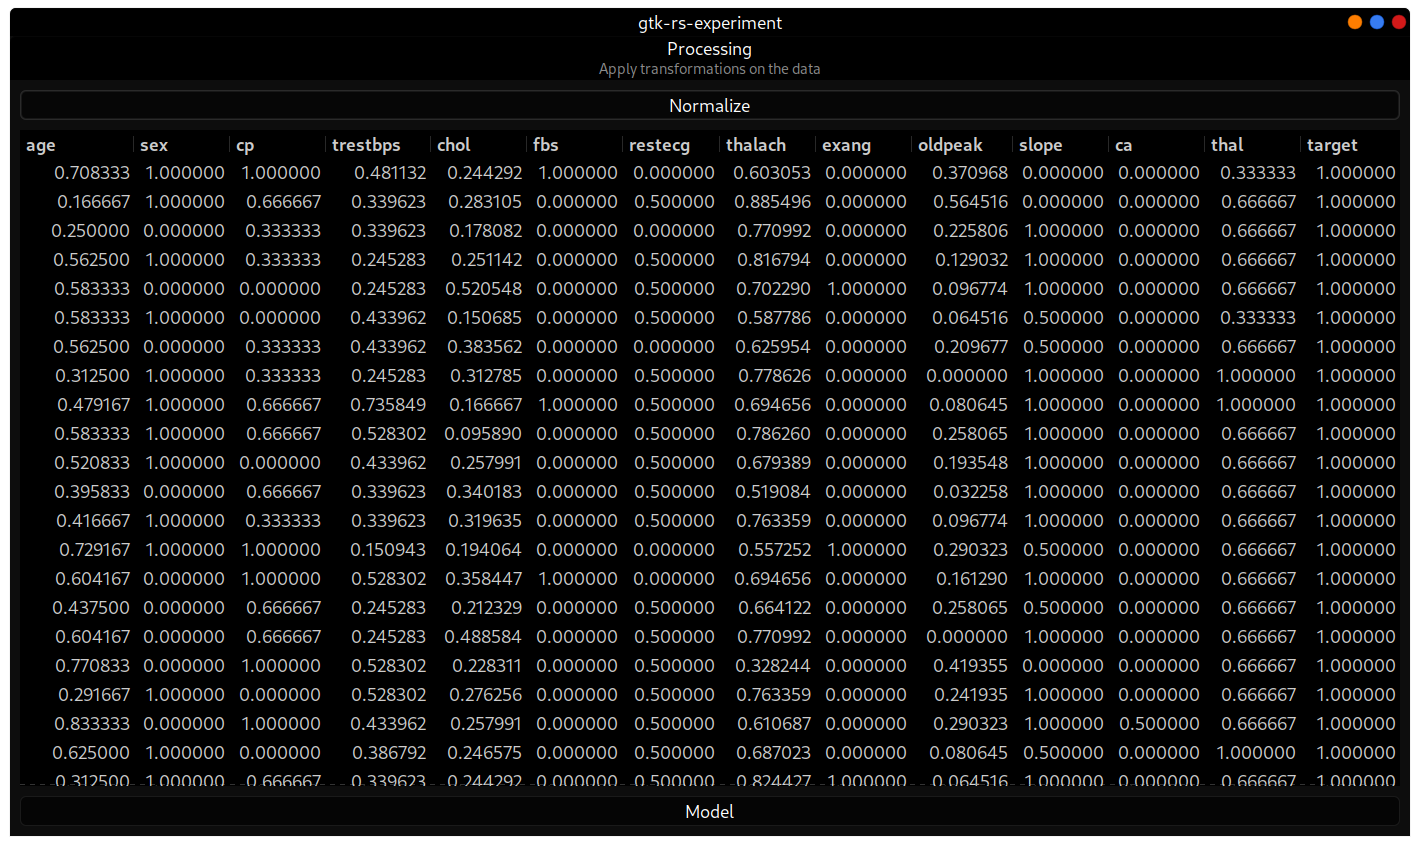
\includegraphics[width=120mm]{preprocessing}
\caption{Preproccessing Page}
\label{fig:preprocessing}
\end{figure}

\begin{figure}[h]
\centering
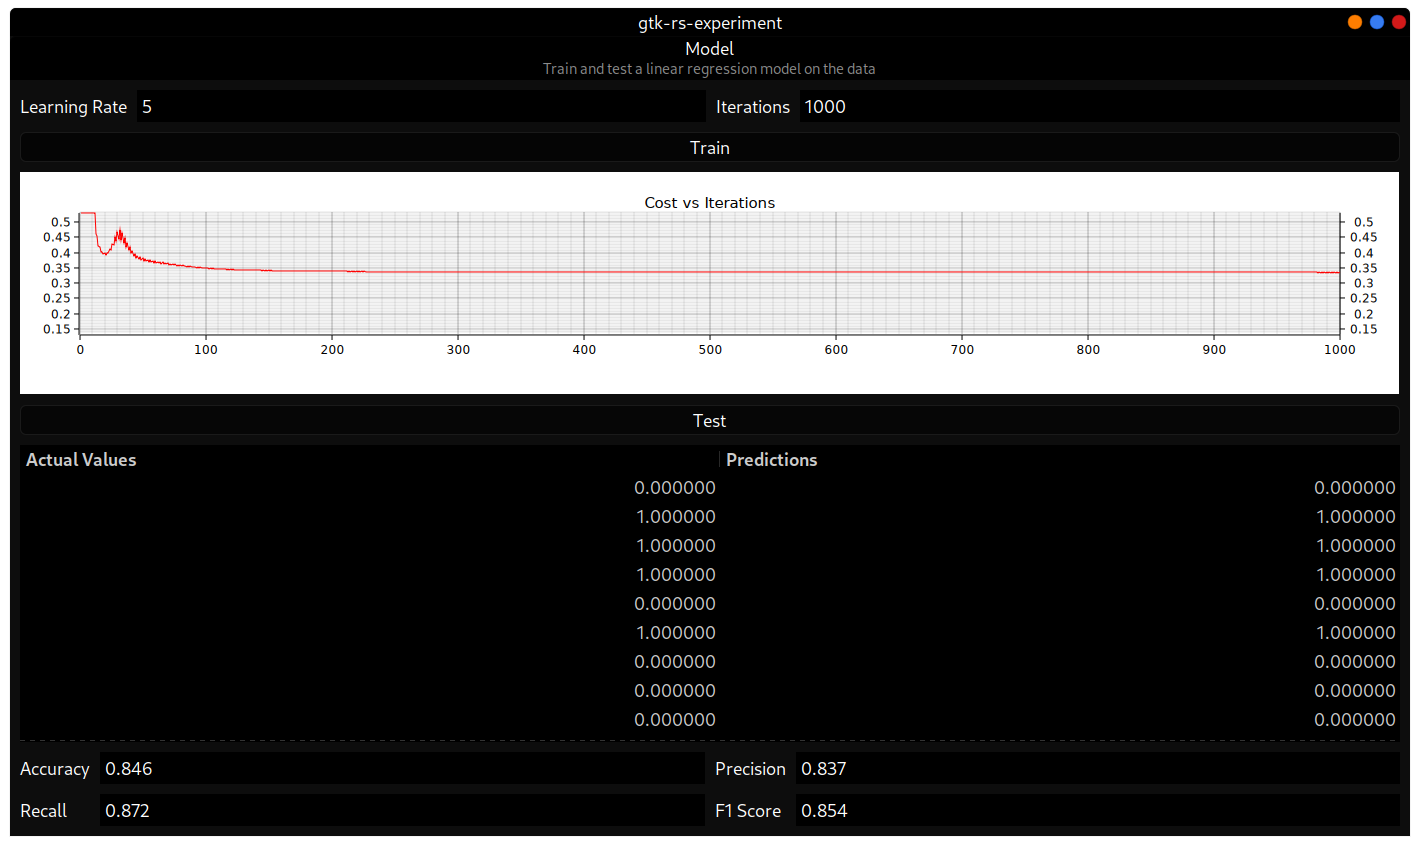
\includegraphics[width=120mm]{model}
\caption{Model Page}
\label{fig:model}
\end{figure}

\section{Analyzing the results}

The results of various values of the hyperparameters, learning rate and
iterations are show in table \ref{table:hyperparams}.

\begin{table}[h]
  \centering
  \begin{tabular}{| p{2cm} | p{2cm} || p{2cm} | p{2cm} | p{2cm} | p{2cm} |}
    \hline
    LR & Iterations & Accuracy & Precision & Recall & F1-Score \\
    \hline
    0.1 & 100  & 79.1\% & 90.2\% & 76.7\% & 82.9\%  \\
    0.1 & 1000 & 80.2\% & 90.2\% & 78.0\% & 83.6\%  \\
    1   & 100  & 80.1\% & 90.2\% & 78.0\% & 83.6\%  \\
    1   & 1000 & 83.5\% & 92.2\% & 81.0\% & 86.2\%  \\
    10  & 100  & 74.2\% & 68.6\% & 83.3\% & 75.3\%  \\
    10  & 1000 & 76.9\% & 70.6\% & 85.7\% & 77.4\%  \\
    \hline
  \end{tabular}
\caption{Metrics for various hyperparameters}
\label{table:hyperparams}
\end{table}

As we can see, the model with the learning rate of 1 and 1000 iterations
performs the best. The learning rate of 0.1 is too slow and it takes 1000 to
match the performance of the (1, 1000) model. The learning rate of 10 is too
fast which is also apparent from it's cost vs iterations graph. Ideally, we'd
like a mechanism that reduces the learning rate whenever the cost stops
decreasing. This is known as an ``adaptive learning rate''.

\section{Setup}

Regardless of the operating system you're on you might need a dataset to test
this on. The app only supports datasets with numeric columns so other datasets
might crash the app.

\begin{enumerate}
  \item{Go to \href{https://raw.githubusercontent.com/ArchitBhonsle/gtk-rs-experiment/main/data/heart.csv}{this}
        link.}
  \item{Right click on the page and select ``Save as''} and save it in the location of you choice.
\end{enumerate}

\subsection{Linux}

\begin{enumerate}
  \item{Go to \href{https://github.com/ArchitBhonsle/gtk-rs-experiment/blob/main/linux-executable?raw=true}{this}
        link.}
  \item{Right click on the page and select ``Save as'' and save it in the location of you choice.}
  \item{Double click on the downloaded executable.}
\end{enumerate}

\subsection{Windows}

\begin{enumerate}
  \item{Go \href{https://download-directory.github.io/}{here}.}
  \item{Input this link: \url{https://github.com/ArchitBhonsle/gtk-rs-experiment/windows-package} and press Enter. This will download the folder.}
  \item{In this folder double click on the \texttt{gtk-rs-experiment.exe}.}
\end{enumerate}

\end{document}
